\chapter{由熵與能量定義溫度}

\lectureoverview{溫度最初是作為換算因子出現，用來將人類溫度計的讀值換算成微觀能量單位。將熱力學熵相應地換算為無量綱的統計熵後，我們以一族由單一參數標記的機率分布描述平衡態。導數\(dE/dS\)於是定義了溫度，而前兩條定律則說明，為何溫差會決定能量流動的方向。}

\section{換算因子與人類使用的單位}

物理學中的許多常數都是換算因子。光速可將距離換算成時間：
\begin{equation}
 t=\frac{x}{c}.
\end{equation}
如果距離和時間以相容的單位測量，就可以令\(c=1\)。這不會使任何物理效應消失；只是把兩種測量改用同一個尺度表示。

波茲曼常數具有相同的性質。它將人類尺度溫度計所測得的溫度換算成能量。「\emph{人類尺度}」這個形容詞很重要。選用這類單位，是因為宏觀儀器能夠產生並分辨相應的溫度，而不是因為微觀動力學特別偏好這些單位。

攝氏溫標是將標準壓力下水的冰點與沸點之間的溫差分成一百等分而定義的。開爾文的刻度間隔大小相同，但將零點定在絕對零度。若改用另一種物質、另一段溫差或華氏度，數值會改變，物理則不會改變。

\begin{classroomqa}
\audiencequestion{華氏溫標早在十七世紀就已經建立了嗎？}
\lecturerresponse{這裡不需要知道確切日期。重點是，這類溫標都是依據人們能夠製備和測量的溫度來設計的。每一度的大小是約定出來的，並非由微觀尺度決定。
\lecturetimestamp{00:01:34--00:01:50}}
\end{classroomqa}

這些溫標創立時，實驗尚無法探知熱的分子起源。宏觀溫度計可以測出一度的變化，卻無法測量單一分子的能量。因此，在人們尚未知道溫度從根本上是一種能量尺度之前，先訂出溫度單位是很自然的事。

\section{為什麼溫度的單位是能量}

考慮稀薄的單原子氣體。就此處的討論而言，稀薄表示可以忽略分子間的交互作用能。在熱平衡下，能量均分定理指出，每個平動二次自由度所分配到的能量為波茲曼常數乘以\(T_{\mathrm K}/2\)。在三維空間中，
\begin{equation}
 \left\langle E_{\mathrm{kin}}\right\rangle
 =\frac{3}{2}k_{\mathrm B}T_{\mathrm K}.
 \label{eq:sm2-equipartition-kelvin}
\end{equation}
因子三計算的是沿\(x\)、\(y\)和\(z\)方向的運動。二分之一因子則來自二次動能。

這個關係並非某一種分子所獨有。在平衡的氦與氧混合氣體中，每個可自由平動的粒子，其質心動能平均值都相同，儘管較重的粒子移動得較慢。由於
\begin{equation}
 E_{\mathrm{kin}}=\frac{1}{2}mv^2,
\end{equation}
特徵能量相同，就意味著\(v\propto m^{-1/2}\)。

這個想法還可以延伸到一個刻意極端的例子。將保齡球懸浮在流體中，並讓整個系統達到平衡。保齡球的布朗平動自由度，與分子遵循相同的能量尺度。球的速度極小，是因為它的質量極大；但溫度比較的是能量尺度，而非速度。

室溫下，\(T_{\mathrm K}\)約為\(300\,\mathrm K\)；相較之下，單一微觀自由度的能量以焦耳計極小。因此，換算因子也非常小：
\begin{equation}
 k_{\mathrm B}\simeq 1.38\times10^{-23}\,
 \mathrm{J\,K^{-1}}.
 \label{eq:sm2-boltzmann-value}
\end{equation}
這個尺度與亞佛加厥常數的關係並非巧合，而是彼此相連：
\begin{equation}
 R=N_{\mathrm A}k_{\mathrm B}.
\end{equation}
氣體常數\(R\)描述一莫耳粒子的尺度，而\(k_{\mathrm B}\)描述每個微觀組成粒子所對應的尺度。

基本公式中反覆出現\(k_{\mathrm B}T_{\mathrm K}\)這個組合。因此，定義
\begin{equation}
 T\equiv k_{\mathrm B}T_{\mathrm K}.
 \label{eq:sm2-energy-temperature}
\end{equation}
會更加簡潔。從現在起，\(T\)本身就以能量為單位，而
\eqref{eq:sm2-equipartition-kelvin}則變為
\begin{equation}
 \left\langle E_{\mathrm{kin}}\right\rangle=\frac{3}{2}T.
 \label{eq:sm2-equipartition-natural}
\end{equation}
若能量以焦耳為單位，溫度也就以焦耳為單位；若能量以電子伏特為單位，溫度也就以電子伏特為單位。自然界並沒有一種稱為「溫度單位」的新單位。

\section{熵的兩種慣例}

熵也有相應的換算。宏觀熱力學是從熱機分析發展而來。卡諾提出了關鍵的熱機推理；克勞修斯後來引入熱力學熵，並以\(S\)表示。在本書使用的記號中，我們將這個宏觀量記為\(S_{\mathrm C}\)。它的單位是能量除以溫度計所用的溫度單位，例如焦耳每開爾文。

統計熵是無量綱的。對離散分布而言，
\begin{equation}
 S=-\sum_i p_i\log p_i.
 \label{eq:sm2-statistical-entropy}
\end{equation}
使用自然對數時，公平二選一的熵為\(\log2\)；使用以二為底的對數時，相同的熵量稱為一位元。兩種熵的慣例之間有如下關係：
\begin{equation}
 S=\frac{S_{\mathrm C}}{k_{\mathrm B}},
 \qquad
 S_{\mathrm C}=k_{\mathrm B}S.
 \label{eq:sm2-entropy-conversion}
\end{equation}
宏觀量以\(\mathrm{J\,K^{-1}}\)為單位時，即使數值不大，也會對應到極大的無量綱熵，因為它計算的是分散在極大量微觀組成粒子中的資訊。

方程式\eqref{eq:sm2-energy-temperature}和
\eqref{eq:sm2-entropy-conversion}確立了全書採用的慣例：
\[
 [T]=[\text{energy}],
 \qquad
 [S]=1.
\]
在接下來的公式中，可以不寫出波茲曼常數；只要分別將\(T\)換成\(k_{\mathrm B}T_{\mathrm K}\)，並將\(S\)換成\(S_{\mathrm C}/k_{\mathrm B}\)，就能恢復它。

\begin{classroomqa}
\audiencequestion{除去因子\(3/2\)，新定義的溫度不就是以焦耳為單位的能量嗎？}
\lecturerresponse{如果選用焦耳作為能量單位，那麼確實如此。焦耳是MKS制中的\(\mathrm{kg\,m^2\,s^{-2}}\)單位。也可以改用電子伏特或其他能量單位；此時溫度就必須以相同的單位表示。因子\(3/2\)屬於理想氣體這個例子，並非溫度定義的一部分。
\lecturetimestamp{00:15:49--00:16:45}}
\end{classroomqa}

\begin{classroomqa}
\audiencequestion{如果黑板上指定的是開爾文，那麼\(k_{\mathrm B}\)不就是一個確定的常數嗎？}
\lecturerresponse{只有在溫度與能量所用的單位都指定之後，它的數值才確定。若將開爾文改成華氏度，或將焦耳改成電子伏特，數值就會改變。這正是換算因子隨單位而變的情形。
\lecturetimestamp{00:16:46--00:18:33}}
\end{classroomqa}

\begin{classroomqa}
\audiencequestion{波茲曼常數的數值是由實驗測定的嗎？}
\lecturerresponse{是的。歷史上，測定波茲曼常數需要原子及其數密度的微觀資訊。波茲曼早在這些量尚未被精確測定之前，就已理解分子能量與溫度的關係；這有如牛頓在重力常數尚未被精確測量之前，就已知道它所扮演的角色。
\lecturetimestamp{00:18:46--00:20:00}}
\end{classroomqa}

\section{平衡是一種統計狀態}

單位換算仍未定義溫度。觸摸高溫物體所帶來的感受，能提供有用的生物學直覺；但溫度是由能量和熵導出的物理量。

設想一個系統與一個宏觀條件固定的大環境接觸，能量可以在兩者之間傳遞。如果系統一開始的能量過多，平均而言就會失去能量；若能量不足，平均而言就會獲得能量。熱平衡時，微觀交換仍持續發生，但兩個方向都沒有淨平均能量流。

令\(i\)表示系統的一個精確微觀狀態，並以\(E_i\)表示該狀態的能量。平衡並不表示系統固定在某一個狀態。系統與環境的交互作用會不斷改變微觀狀態，因此我們為每種可能性指定一個機率\(P_i\)。基本關係如下：
\begin{align}
 \sum_i P_i &=1,
 \label{eq:sm2-normalization}\\
 \sum_i P_iE_i &=\overline E,
 \label{eq:sm2-mean-energy}\\
 S&=-\sum_iP_i\log P_i.
 \label{eq:sm2-equilibrium-entropy}
\end{align}
\(\overline E\)上方的橫線強調子系統的能量會發生漲落。一次測量可能得到某個值，下一次則可能得到另一個值；重複測量後，結果會符合某個分布，其平均值為\eqref{eq:sm2-mean-energy}。

\begin{figure}[t]
\centering
\includegraphics[width=0.82\textwidth]{lecture_02_figure_02.png}
\caption{黑板上的歸一化條件與平均能量：
\(\sum_iP(i)=1\)和\(\sum_iP(i)E(i)=\langle E\rangle\)。}
\lectureframe{00:24:10}
\end{figure}

\section{以平均能量標記的一族分布}

平衡分布會隨平均能量顯著改變。把一壺水放在爐子上，\(\overline E\)會上升；把它放進雪中，\(\overline E\)會下降。機率也會隨之改變。因此，平衡應視為一族由單一參數標記的分布，而非單一分布：
\begin{equation}
 P_i(\overline E).
 \label{eq:sm2-family}
\end{equation}
族中的每個分布都滿足
\begin{align}
 \sum_iP_i(\overline E)&=1,
 \label{eq:sm2-family-normalization}\\
 \sum_iP_i(\overline E)E_i&=\overline E.
 \label{eq:sm2-family-mean}
\end{align}

\begin{figure}[t]
\centering
\includegraphics[width=0.88\textwidth]{lecture_02_figure_03.png}
\caption{引入\(P(i,\overline E)\)。介紹這一族分布時，先前的歸一化、平均能量與熵方程式仍保留在黑板上。}
\lectureframe{00:26:29}
\end{figure}

在示意圖中，將狀態依\(E_i\)遞增排列。如此一來，橫軸既可讀作索引\(i\)，也可讀作相應的能量。平均能量較高時，機率權重會移向較右側的狀態。每條曲線的總面積都必須為一。

\begin{figure}[t]
\centering
\includegraphics[width=0.88\textwidth]{lecture_02_figure_04.png}
\caption{數個示意分布\(P(i,\overline E)\)。機率權重偏向右側的曲線，其平均能量較高；每條曲線仍各自歸一化。}
\lectureframe{00:28:40}
\end{figure}

\begin{figure}[t]
\centering
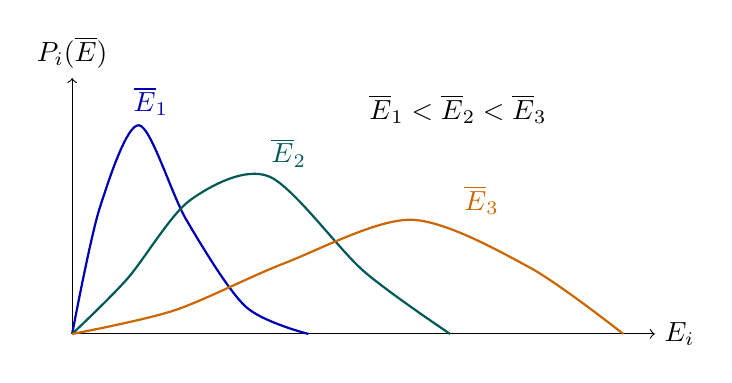
\begin{tikzpicture}[x=1cm,y=1cm]
\draw[->] (0,0) -- (7.4,0) node[right] {$E_i$};
\draw[->] (0,0) -- (0,3.25) node[above] {$P_i(\overline E)$};
\draw[thick,blue!70!black]
  plot[smooth] coordinates {(0,0) (0.35,1.6) (0.85,2.65) (1.45,1.45)
  (2.2,0.35) (3.0,0)};
\draw[thick,teal!70!black]
  plot[smooth] coordinates {(0,0) (0.7,0.7) (1.5,1.7) (2.5,2.0)
  (3.7,0.8) (4.8,0)};
\draw[thick,orange!80!black]
  plot[smooth] coordinates {(0,0) (1.3,0.3) (2.7,0.9) (4.3,1.45)
  (5.8,0.85) (7.0,0)};
\node[blue!70!black] at (1.0,2.95) {\(\overline E_1\)};
\node[teal!70!black] at (2.75,2.3) {\(\overline E_2\)};
\node[orange!80!black] at (5.2,1.7) {\(\overline E_3\)};
\node at (4.9,2.85) {\(\overline E_1<\overline E_2<\overline E_3\)};
\end{tikzpicture}
\caption{黑板草圖的清晰版本。曲線不必具有圖中這些精確形狀；這裡只用到歸一化條件，以及各曲線平均能量的大小順序。}
\end{figure}

\begin{classroomqa}
\audiencequestion{這個記號是否形成循環定義？平均能量是從分布計算而得，分布卻又以平均能量標記。}
\lecturerresponse{先從經驗上選定一族由單一參數標記的平衡分布。族中的每個分布都有一個平均能量。若不同分布的平均能量各不相同，就可以用平均能量作為標記這一族的參數。這個記號尚未推導出這一族分布；稍後將由波茲曼分布給出推導。
\lecturetimestamp{00:28:35--00:29:44}}
\end{classroomqa}

\begin{classroomqa}
\audiencequestion{為什麼說平均能量，而不說總能量？}
\lecturerresponse{子系統正與熱浴交換能量；例如，氣體容器的壁具有透熱性，因此周圍的大氣可作為熱浴。子系統的瞬時能量會漲落。多次測量會得到一個分布，而\(\overline E\)是這些測量結果的平均值。由子系統和熱浴組成的較大封閉系統，其能量仍可能固定。
\lecturetimestamp{00:29:46--00:30:56}}
\end{classroomqa}

\begin{classroomqa}
\audiencequestion{不同的微觀狀態能否具有相同的能量？不同的分布能否具有相同的平均能量？}
\lecturerresponse{兩者都有可能。只施加平均能量這項限制，仍容許許多種分布；因此，要選出這一特殊的單參數平衡分布族，還需要額外的物理論證。稍後會推導它的來源及其波茲曼形式。不同微觀狀態具有相同能量，則是另一個稱為簡併的問題。
\lecturetimestamp{00:30:58--00:32:22}}
\end{classroomqa}

\subsection{狀態標記、簡併與關聯}

有幾個容易混淆的概念，必須彼此區分。

第一，許多機率分布可能具有相同的平均能量。單靠平均能量限制，無法得出這一族由單一參數標記的平衡分布；它是系統達到平衡時所選出的特定分布族。稍後會將其形式辨認為波茲曼分布。

第二，不同的微觀狀態可能具有相同的能量，這稱為簡併。黑板上的討論暫時忽略能量完全相同的情形，使狀態能依能量明確排序。系統具有對稱性時，簡併其實很常見，但這不會造成概念上的困難：保留狀態標記\(i\)，允許\(E_i\)取相同值，並對所有狀態求和。

第三，關聯並非簡併的另一種說法。關聯涉及兩個隨機量的聯合分布，探討得知其中一個量後，另一個量的機率是否會改變。在同一份微觀狀態列表中，互斥的標記\(i\)和\(j\)本身並不是正在計算關聯的兩個隨機變數。

\begin{classroomqa}
\audiencequestion{這個推導是否假設不同的\(i\)態彼此獨立？如果其中兩個態彼此相關，該怎麼辦？}
\lecturerresponse{狀態標記是單一微觀隨機變數的一個可能取值。獨立性與關聯性需要兩個具有聯合分布的變數，因此這些術語不能直接用來描述此列表中的兩個替代標記。不同狀態具有相同能量，則是簡併問題。
\lecturetimestamp{00:32:23--00:33:22}}
\end{classroomqa}

\begin{classroomqa}
\audiencequestion{如果兩個不同狀態的能量完全相同，該怎麼辦？}
\lecturerresponse{這就是簡併。為了繪製目前的圖，我們採用一項簡化假設：任意兩個狀態的能量都不相同，並依能量遞增排列。後面的機率公式不需要這項假設；簡併的狀態只要分別計數即可。
\lecturetimestamp{00:33:23--00:34:04}}
\end{classroomqa}

\begin{classroomqa}
\audiencequestion{索引\(i\)的意義是任意的嗎？}
\lecturerresponse{微觀狀態本身並非任意：每個狀態都指定了精確描述系統所需的所有位置、動量或其他資料。任意的是狀態的名稱，因此在圖中我們選擇依能量遞增的順序標記狀態。
\lecturetimestamp{00:34:06--00:35:15}}
\end{classroomqa}

\section{熵成為能量的函數}

平衡分布族中的每個成員都有熵。將\eqref{eq:sm2-family}代入\eqref{eq:sm2-equilibrium-entropy}，得到
\begin{equation}
 S(\overline E)
 =-\sum_iP_i(\overline E)\log P_i(\overline E).
 \label{eq:sm2-entropy-energy}
\end{equation}
這不是所有物理系統共用的普適函數；它取決於系統的能譜和平衡分布族。不過，一旦指定了這一族，能量與熵便相互關聯：沿著這一族改變分布時，兩者都會改變。

一般而言，隨著平均能量上升，系統會把機率分散到更多狀態，因此\(S\)通常會隨\(\overline E\)增加。目前先假設兩者的關係是光滑且局部可逆的。雖然例外情形也很重要，但先看簡單情況，就能引出所需的定義。

\section{定義溫度的導數}

問一個具體的問題：若要讓熵增加一個二元選擇的熵量，平均能量需要改變多少？以自然對數為單位，這個熵增量是\(\log2\)。

對於光滑分布族中彼此相鄰的成員，
\begin{equation}
 dE=\frac{dE}{dS}\,dS.
 \label{eq:sm2-differential-identity}
\end{equation}
此時，這個方程式不過是鏈鎖律。然而，它的係數恰好具有溫度所需的量綱與物理作用。

\begin{definition}
以能量為單位的溫度定義為
\begin{equation}
 T\equiv\frac{dE}{dS}.
 \label{eq:sm2-temperature-definition}
\end{equation}
等價地，
\begin{equation}
 dE=T\,dS,
 \qquad
 dS=\frac{1}{T}\,dE.
 \label{eq:sm2-fundamental-differentials}
\end{equation}
\end{definition}

對於一個位元所對應的微小變化，
\begin{equation}
 \Delta E\simeq T\log2.
 \label{eq:sm2-one-bit-energy}
\end{equation}
特別考慮一個位元，只是為了讓導數的意義更具體。任何微小的熵變都遵循相同的局部關係。

\begin{classroomqa}
\audiencequestion{既然熵寫成\(S(E)\)，那麼\(dS/dE\)不是更自然的導數嗎？}
\lecturerresponse{只要兩者的關係在局部可逆，這兩個導數就包含相同資訊：
\[
 \frac{dE}{dS}=\left(\frac{dS}{dE}\right)^{-1}.
\]
依慣例，溫度定義為\(dE/dS\)，而逆溫度則為\(dS/dE=1/T\)。
\lecturetimestamp{00:40:24--00:40:54}}
\end{classroomqa}

這裡只有一個熱力學變數在變化，因此用普通導數就足夠了。若體積、粒子數、磁化強度或其他變數也可變化，就必須使用偏導數，並說明哪些量維持不變。目前的定義是更一般的熱力學幾何中，僅有一個變數變化的情形。

\subsection{為什麼波茲曼常數會消去}

再簡短回顧溫度計所用的單位。利用
\[
 T=k_{\mathrm B}T_{\mathrm K},
 \qquad
 S=\frac{S_{\mathrm C}}{k_{\mathrm B}},
\]
基本關係變為
\begin{align}
 dE
 &=\bigl(k_{\mathrm B}T_{\mathrm K}\bigr)
   d\left(\frac{S_{\mathrm C}}{k_{\mathrm B}}\right)\\
 &=T_{\mathrm K}\,dS_{\mathrm C}.
 \label{eq:sm2-carnot-form}
\end{align}
溫度中含有一個\(k_{\mathrm B}\)因子，熵中則含有它的倒數，兩者正好抵消。這就是為什麼傳統熱力學教材可以不寫出波茲曼常數，直接寫成\eqref{eq:sm2-carnot-form}。

\begin{classroomqa}
\audiencequestion{\(S(E)\)必須可逆嗎？}
\lecturerresponse{不一定。在此處考慮的一般系統中，增加能量通常會使平衡分布變得更廣，並使熵增加，因此\(S(E)\)是單調函數，而且\(T>0\)。能譜有上限的系統可能是反例；其中有些區域的熵會隨能量增加而減少，統計溫度也會是負值。目前先不討論這些情形。
\lecturetimestamp{00:44:30--00:45:57}}
\end{classroomqa}

\section{從抽象導數到熱與冷}

以導數定義溫度雖然普適，仍然相當抽象。我們希望重新得到熟悉的說法：能量會從較熱的物體流向較冷的物體。觸摸高溫表面所感到的疼痛屬於生物學範疇；顏色與物體發出的輻射則取決於光的性質。即使忽略輻射，統計定義也應適用於理想化的氣體。

\begin{classroomqa}
\audiencequestion{高溫物體發出的光，能否作為溫度的基本定義？}
\lecturerresponse{輻射可用來測溫，但這會牽涉光的物理學。統計力學必須能為一盒氣體這類系統定義溫度，而不依賴光學性質。能量交換的方向才是更普遍的判準。
\lecturetimestamp{00:46:42--00:47:20}}
\end{classroomqa}

準備兩個系統\(A\)和\(B\)，讓它們各自先處於平衡態，溫度分別為\(T_A\)和\(T_B\)。起初兩者彼此隔離，接著透過微弱的熱接觸將它們連接起來：這條\emph{細管}允許少量能量來回傳遞，同時不破壞任一子系統的獨立性。

\begin{figure}[t]
\centering
\includegraphics[width=0.88\textwidth]{lecture_02_figure_05.png}
\caption{分別準備好的系統\(A\)和\(B\)，其溫度分別標記為\(T_A\)和\(T_B\)；圖示為考慮微弱熱接觸之前的情形。}
\lectureframe{00:48:55}
\end{figure}

\begin{figure}[t]
\centering
\begin{tikzpicture}[>=Stealth]
\draw[rounded corners,thick,fill=blue!6] (0,0) rectangle (2.6,2.4);
\draw[rounded corners,thick,fill=orange!8] (5.4,0) rectangle (8,2.4);
\draw[thick] (2.6,1.35) -- (5.4,1.35);
\draw[thick] (2.6,1.05) -- (5.4,1.05);
\draw[<->,very thick] (3.15,1.2) -- (4.85,1.2)
  node[midway,above] {\(\delta E\)};
\node at (1.3,1.45) {\Large \(A\)};
\node at (6.7,1.45) {\Large \(B\)};
\node at (1.3,0.65) {\(T_A,S_A,E_A\)};
\node at (6.7,0.65) {\(T_B,S_B,E_B\)};
\node at (4,0.35) {\small weak thermal contact};
\end{tikzpicture}
\caption{能量透過微弱接觸而漲落，同時整個組合系統維持孤立。}
\end{figure}

不失一般性，假設
\begin{equation}
 T_B>T_A.
 \label{eq:sm2-temperature-order}
\end{equation}
根據經驗，\(B\)應會失去能量，而\(A\)應會獲得能量。三項事實可以將這個預期轉化為計算。

\subsection{熵的可加性}

對於兩個微弱耦合的子系統，若兩者的微觀可能性彼此獨立，組合後的可能狀態數便是兩者狀態數的乘積：
\[
 W_{AB}=W_AW_B.
\]
熵是狀態數的對數，因此
\begin{equation}
 S_{\mathrm{tot}}=S_A+S_B.
 \label{eq:sm2-entropy-additivity}
\end{equation}
直接計算乘積分布的夏農熵，也會得到相同結果。

\begin{classroomqa}
\classquestion{為什麼組合系統的熵會相加？}
\lecturerresponse{因為底層可能狀態的數目會相乘，而熵取的是對數：
\(\log(W_AW_B)=\log W_A+\log W_B\)。交互作用微弱，才能將系統描述為兩個子系統，也才能得到這個主要的可加形式。
\lecturetimestamp{00:51:06--00:52:03}}
\end{classroomqa}

\subsection{第一定律與第二定律}

組合系統是孤立的，因此內部交換的能量守恆：
\begin{equation}
 dE_A+dE_B=0,
 \qquad
 dE_B=-dE_A.
 \label{eq:sm2-first-law}
\end{equation}
這就是本例中的第一定律。

此處先將第二定律視為一項公設；稍後會進一步說明其更深層的原因。相連的兩個系統逐漸弛豫到新的平衡態時，
\begin{equation}
 dS_{\mathrm{tot}}=dS_A+dS_B\geq0.
 \label{eq:sm2-second-law}
\end{equation}
嚴格不等式描述系統自發地向平衡態弛豫；在平衡態下，對可逆的一階變化，等號成立。

最後，溫度的定義適用於每個子系統：
\begin{equation}
 dE_A=T_A\,dS_A,
 \qquad
 dE_B=T_B\,dS_B.
 \label{eq:sm2-two-temperatures}
\end{equation}

\begin{figure}[H]
\centering
\includegraphics[width=0.88\textwidth]{lecture_02_figure_06.png}
\caption{黑板推導結尾的兩個子系統關係式：
\(dE_A=T_A\,dS_A\)和\(dE_B=T_B\,dS_B\)。}
\lectureframe{00:54:00}
\end{figure}

\subsection{能量流動的方向}

這些方程式已足以確定淨能量傳遞的方向。將
\(dS_A=dE_A/T_A\)、\(dS_B=dE_B/T_B\)和
\eqref{eq:sm2-first-law}代入\eqref{eq:sm2-second-law}：
\begin{align}
 dS_{\mathrm{tot}}
 &=\frac{dE_A}{T_A}+\frac{dE_B}{T_B}\\
 &=dE_A\left(\frac{1}{T_A}-\frac{1}{T_B}\right)\geq0.
 \label{eq:sm2-flow-sign}
\end{align}
若\(T_B>T_A>0\)，則
\[
 \frac{1}{T_A}-\frac{1}{T_B}>0.
\]
因此，方程式\eqref{eq:sm2-flow-sign}要求
\[
 dE_A>0,
 \qquad
 dE_B<0.
\]
較冷的系統\(A\)會獲得能量，較熱的系統\(B\)則會失去能量。當\(T_A=T_B\)時，一階熵變不偏好任何方向，微觀交換彼此平衡，淨能量流為零。因此，抽象導數\(T=dE/dS\)確實重現了熱與冷在操作上的區別。